%!TEX root=../../main.tex


\subsection{PageRank}

\begin{figure*}
	\begin{subfigure}{0.3\textwidth}
		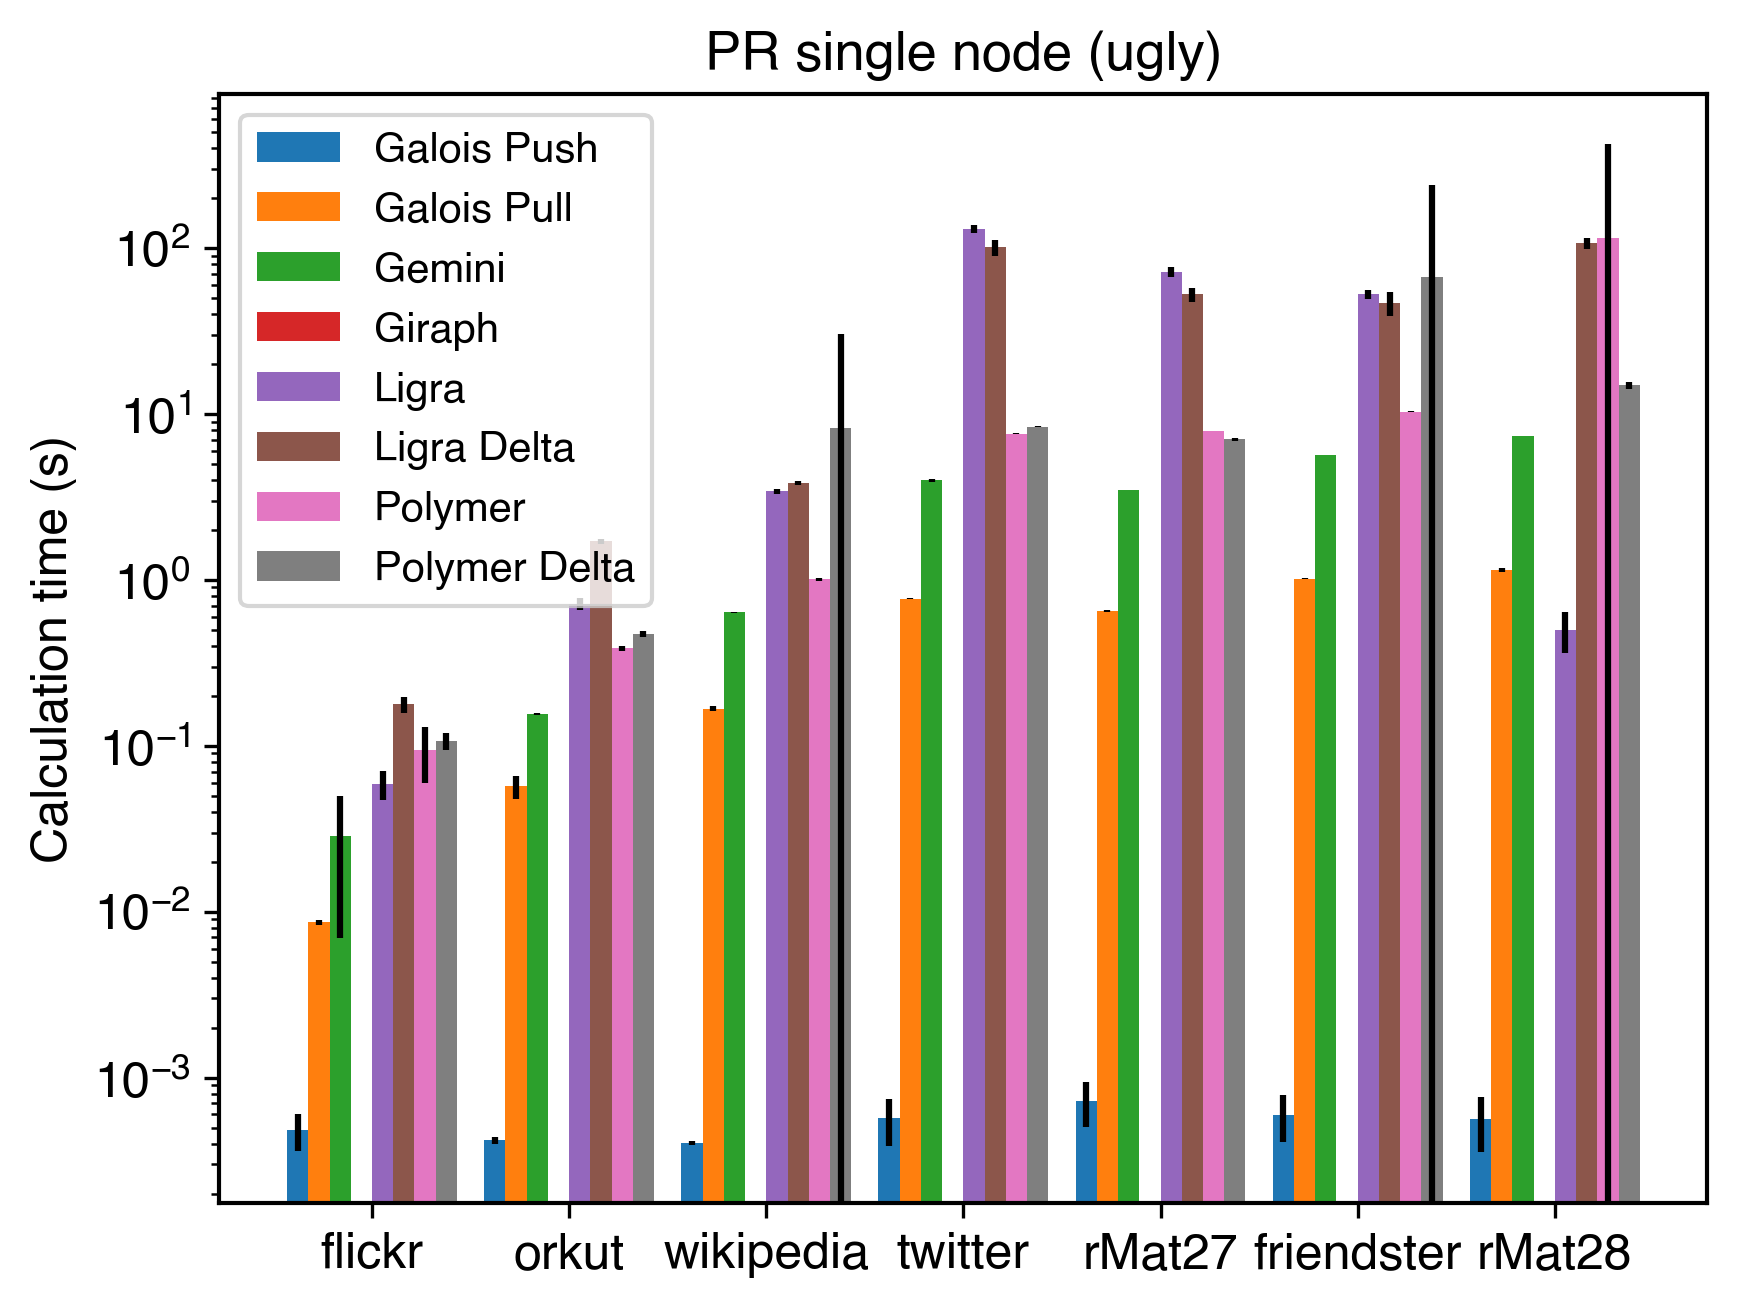
\includegraphics[width=\linewidth]{../../plots/singleNodePR_calcTime.png}
		\caption{Calculation times for PR on a single node}
		\label{fig:singleNodePR_calc}
	\end{subfigure}
	\hfil
	\begin{subfigure}{0.3\textwidth}
		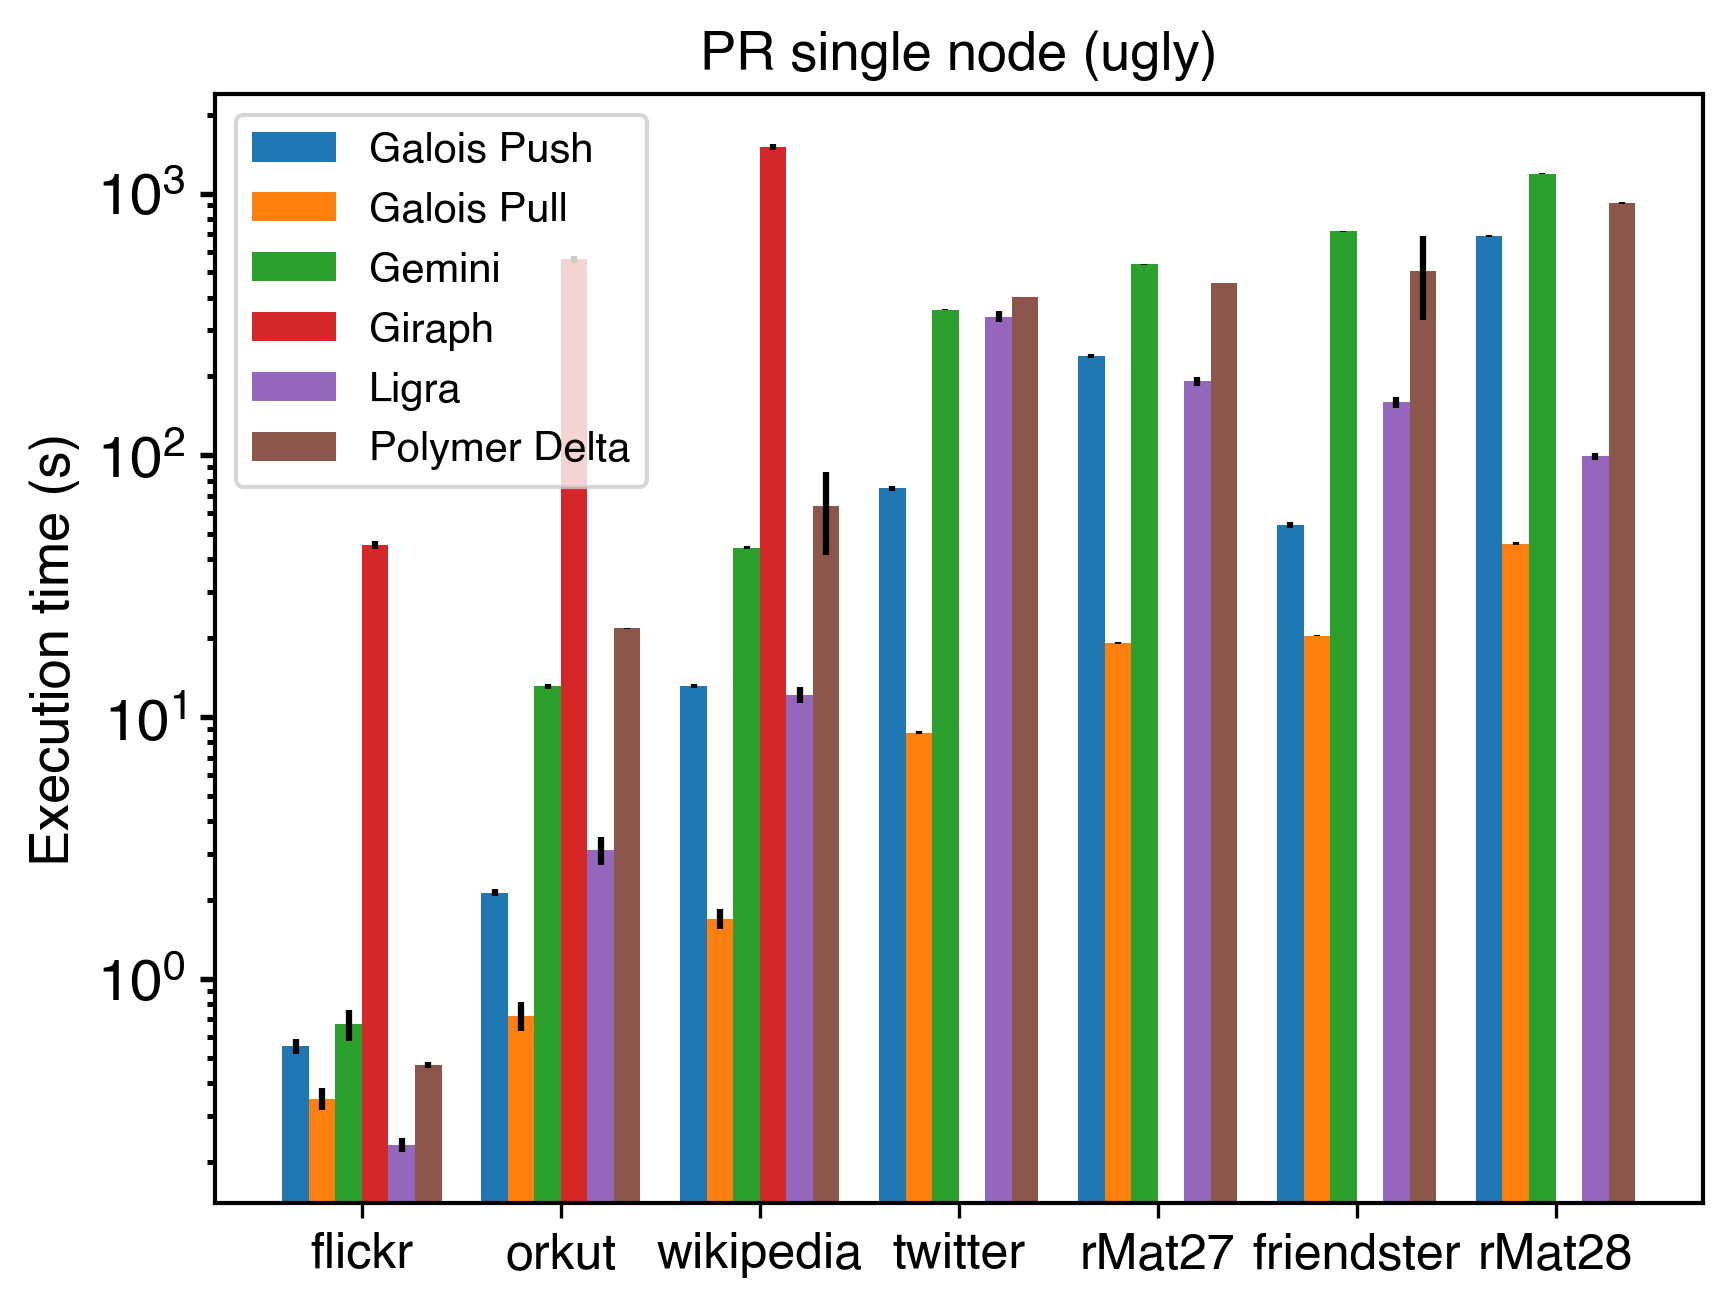
\includegraphics[width=\linewidth]{../../plots/singleNodePR_execTime.png}
		\caption{Execution times for PR on a single node}
		\label{fig:singleNodePR_exec}
	\end{subfigure}
	\hfil
	\begin{subfigure}{0.3\textwidth}
		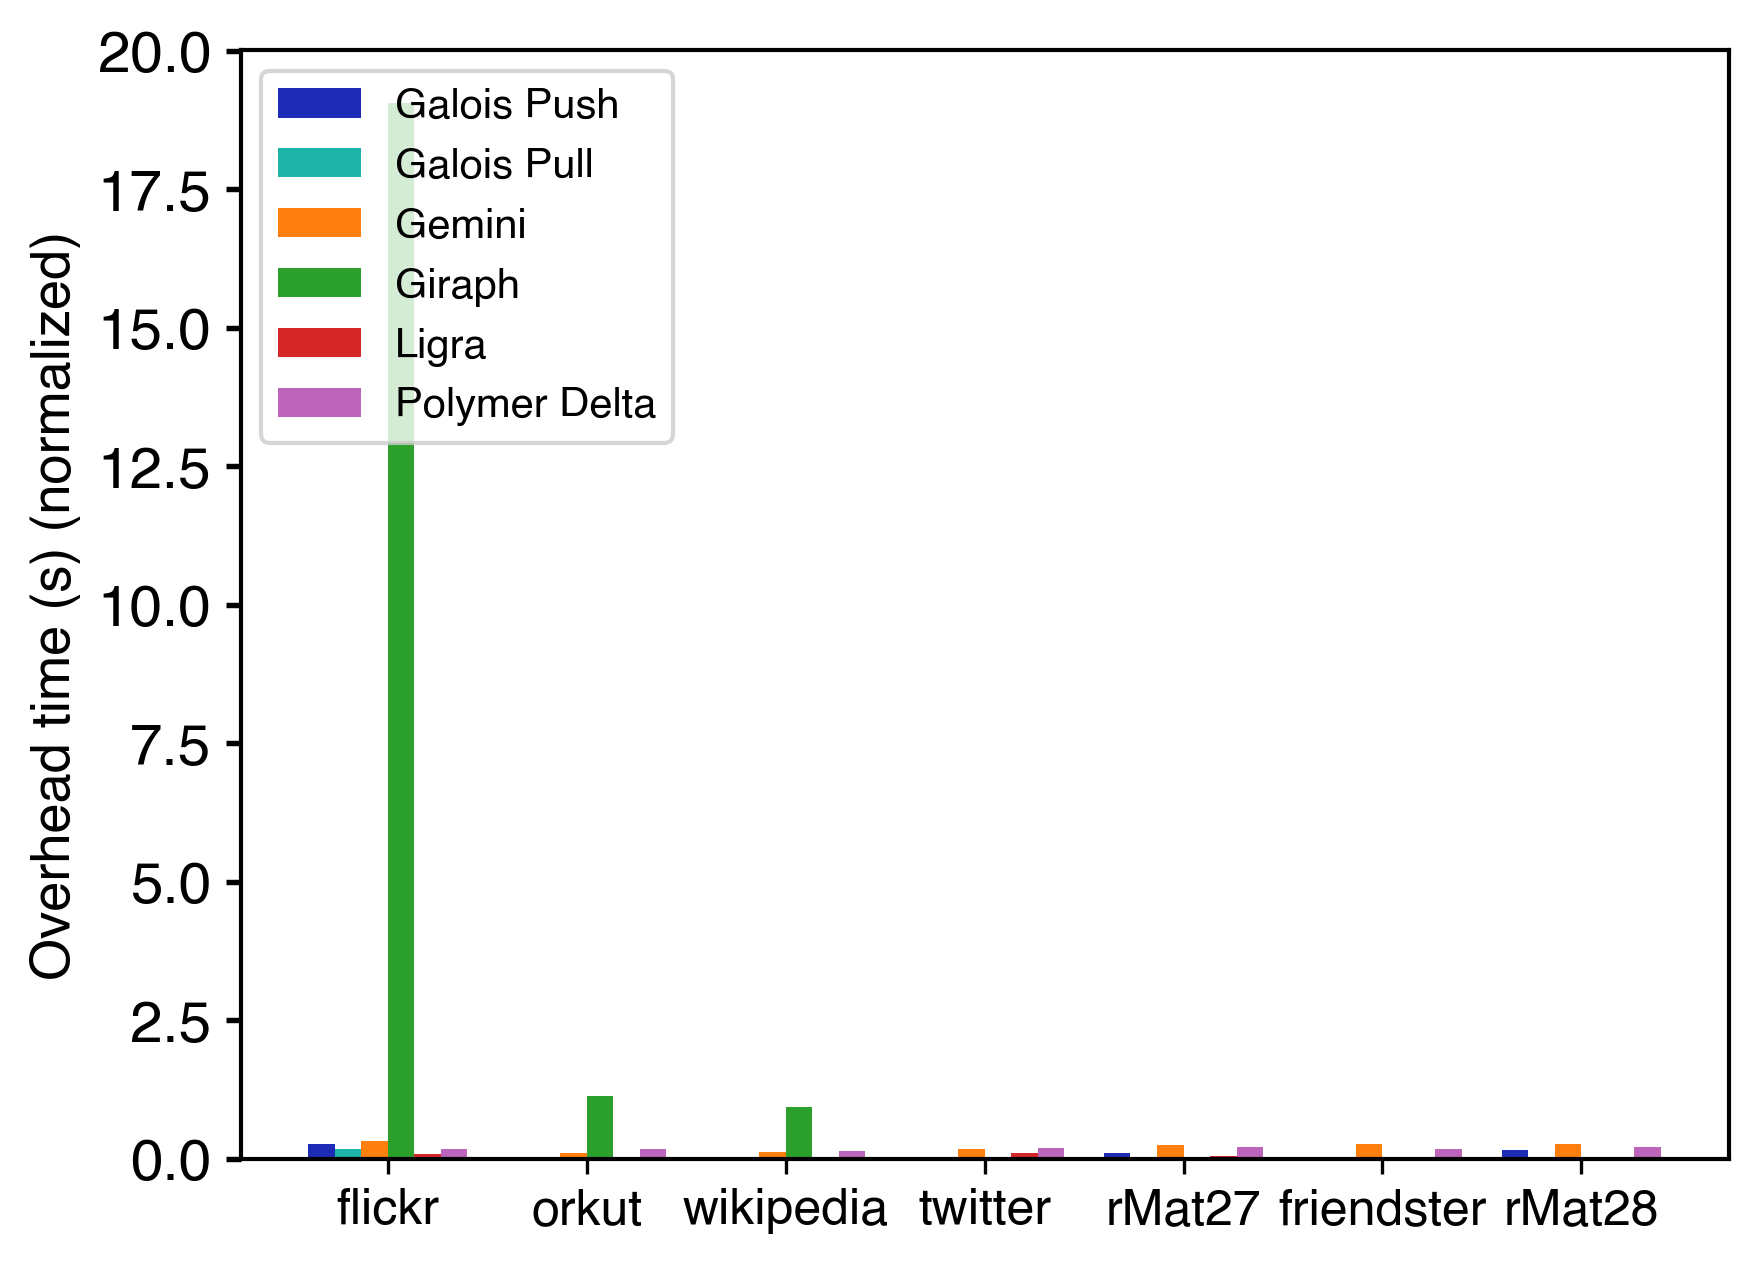
\includegraphics[width=\linewidth]{../../plots/singleNodePR_overheadTimeNormalized.png}
		\caption{Overhead time normalized by the graph size in million edges}
		\label{fig:singleNodePR_overheadNormalized}
	\end{subfigure}
	
	\caption{Average times on a single computation node, black bars represent one standard deviation in our testing}
\end{figure*}




\begin{figure*}
	\begin{subfigure}{0.3\textwidth}
		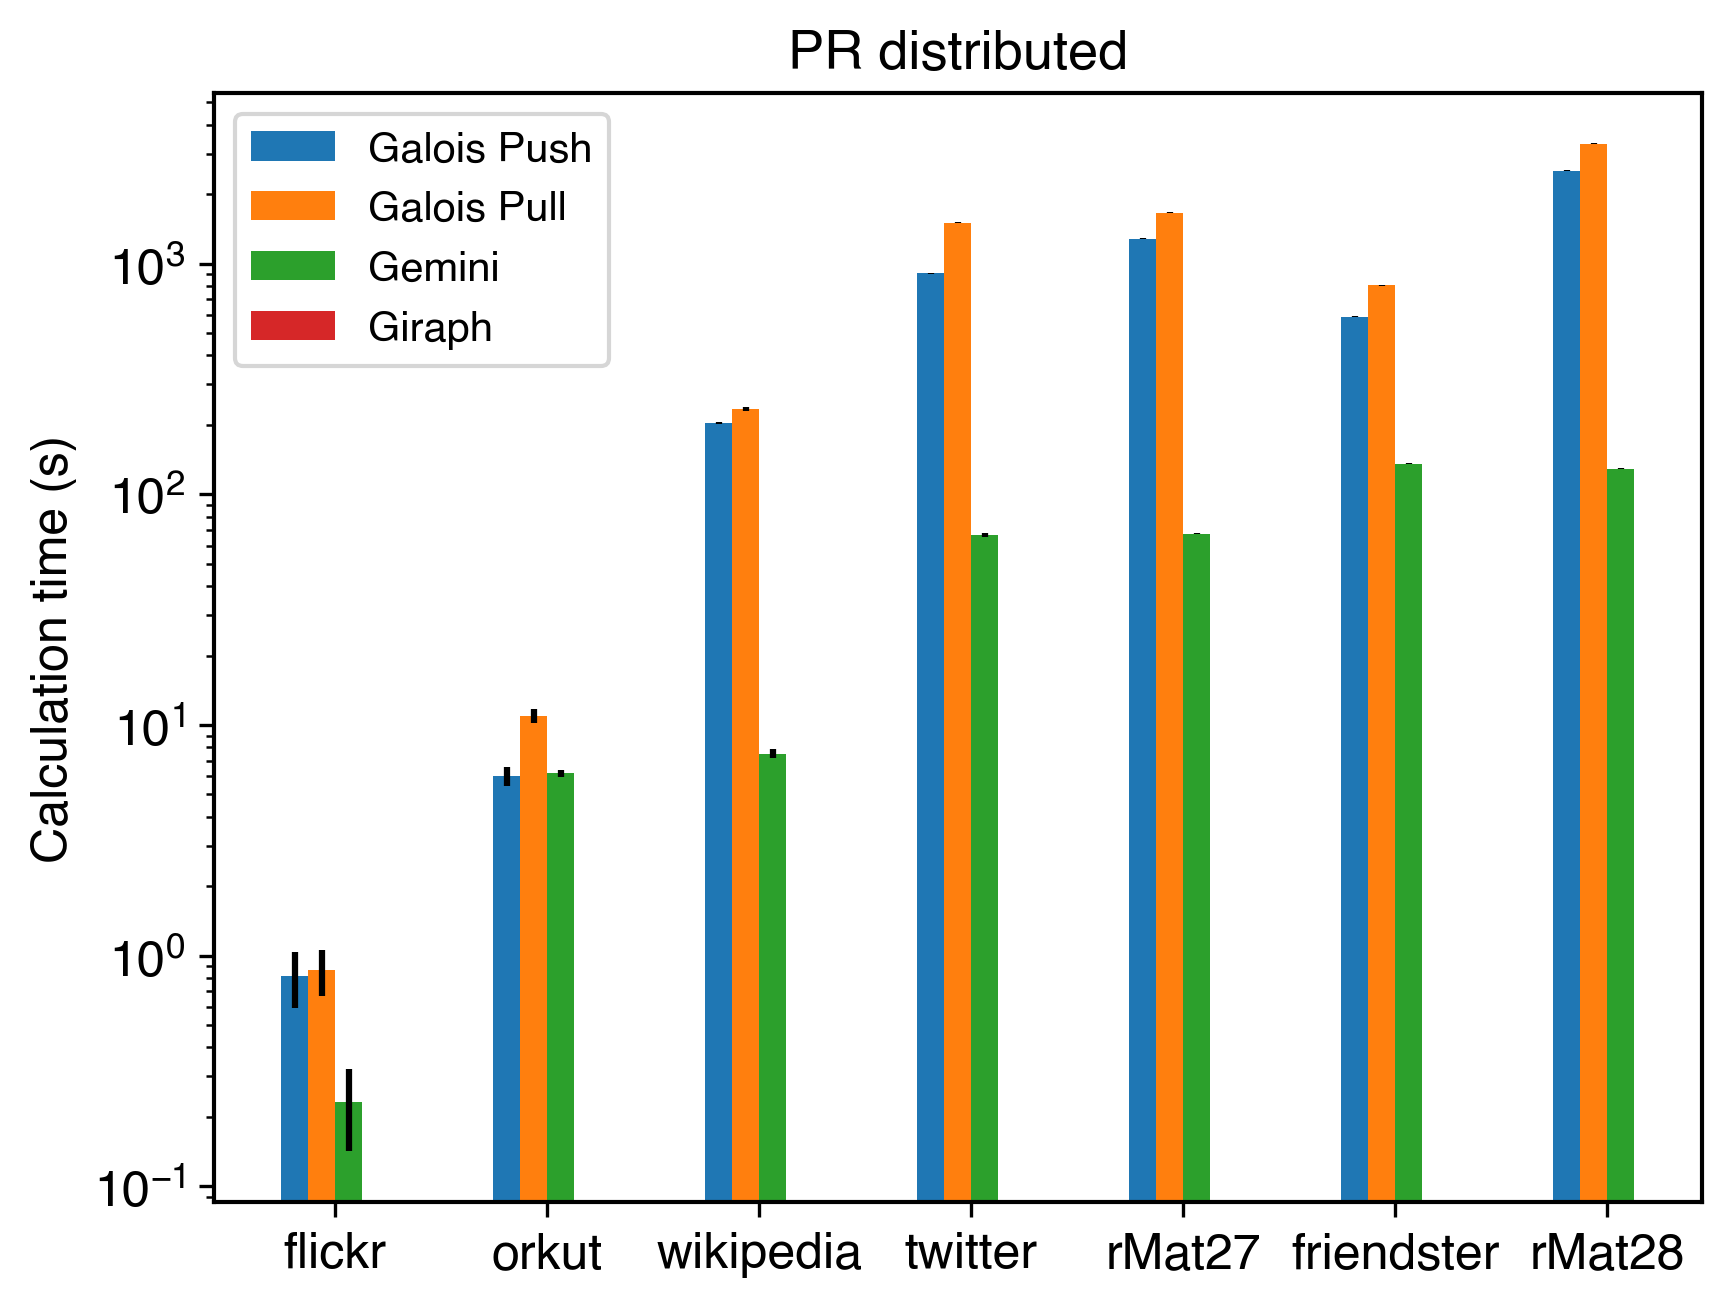
\includegraphics[width=\linewidth]{../../plots/distributedPR_calcTime.png}
		\caption{Calculation times for distributed PR}
		\label{fig:distributedPR_calc}
	\end{subfigure}
	\hfil
	\begin{subfigure}{0.3\textwidth}
		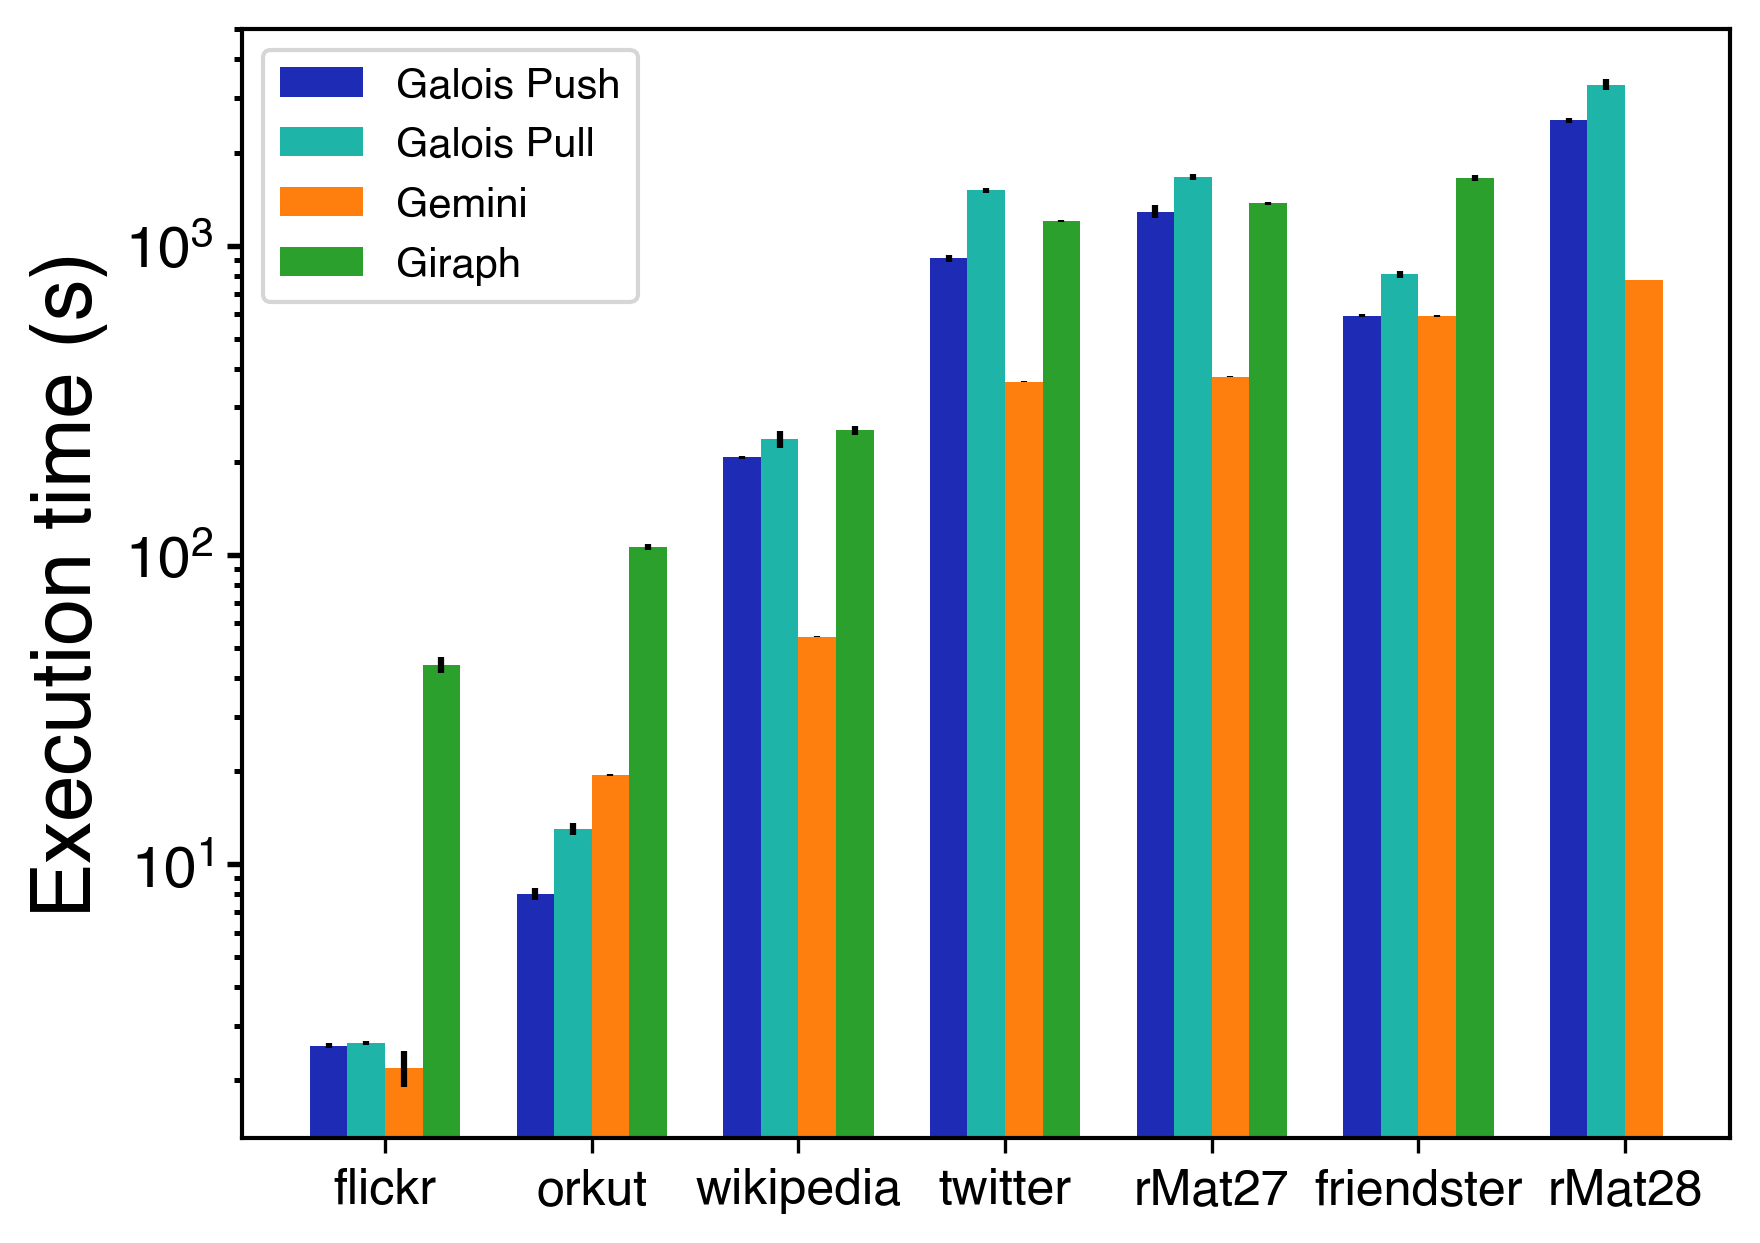
\includegraphics[width=\linewidth]{../../plots/distributedPR_execTime.png}
		\caption{Execution times for distributed PR}
		\label{fig:distributedPR_exec}
	\end{subfigure}
	\hfil
	\begin{subfigure}{0.3\textwidth}
		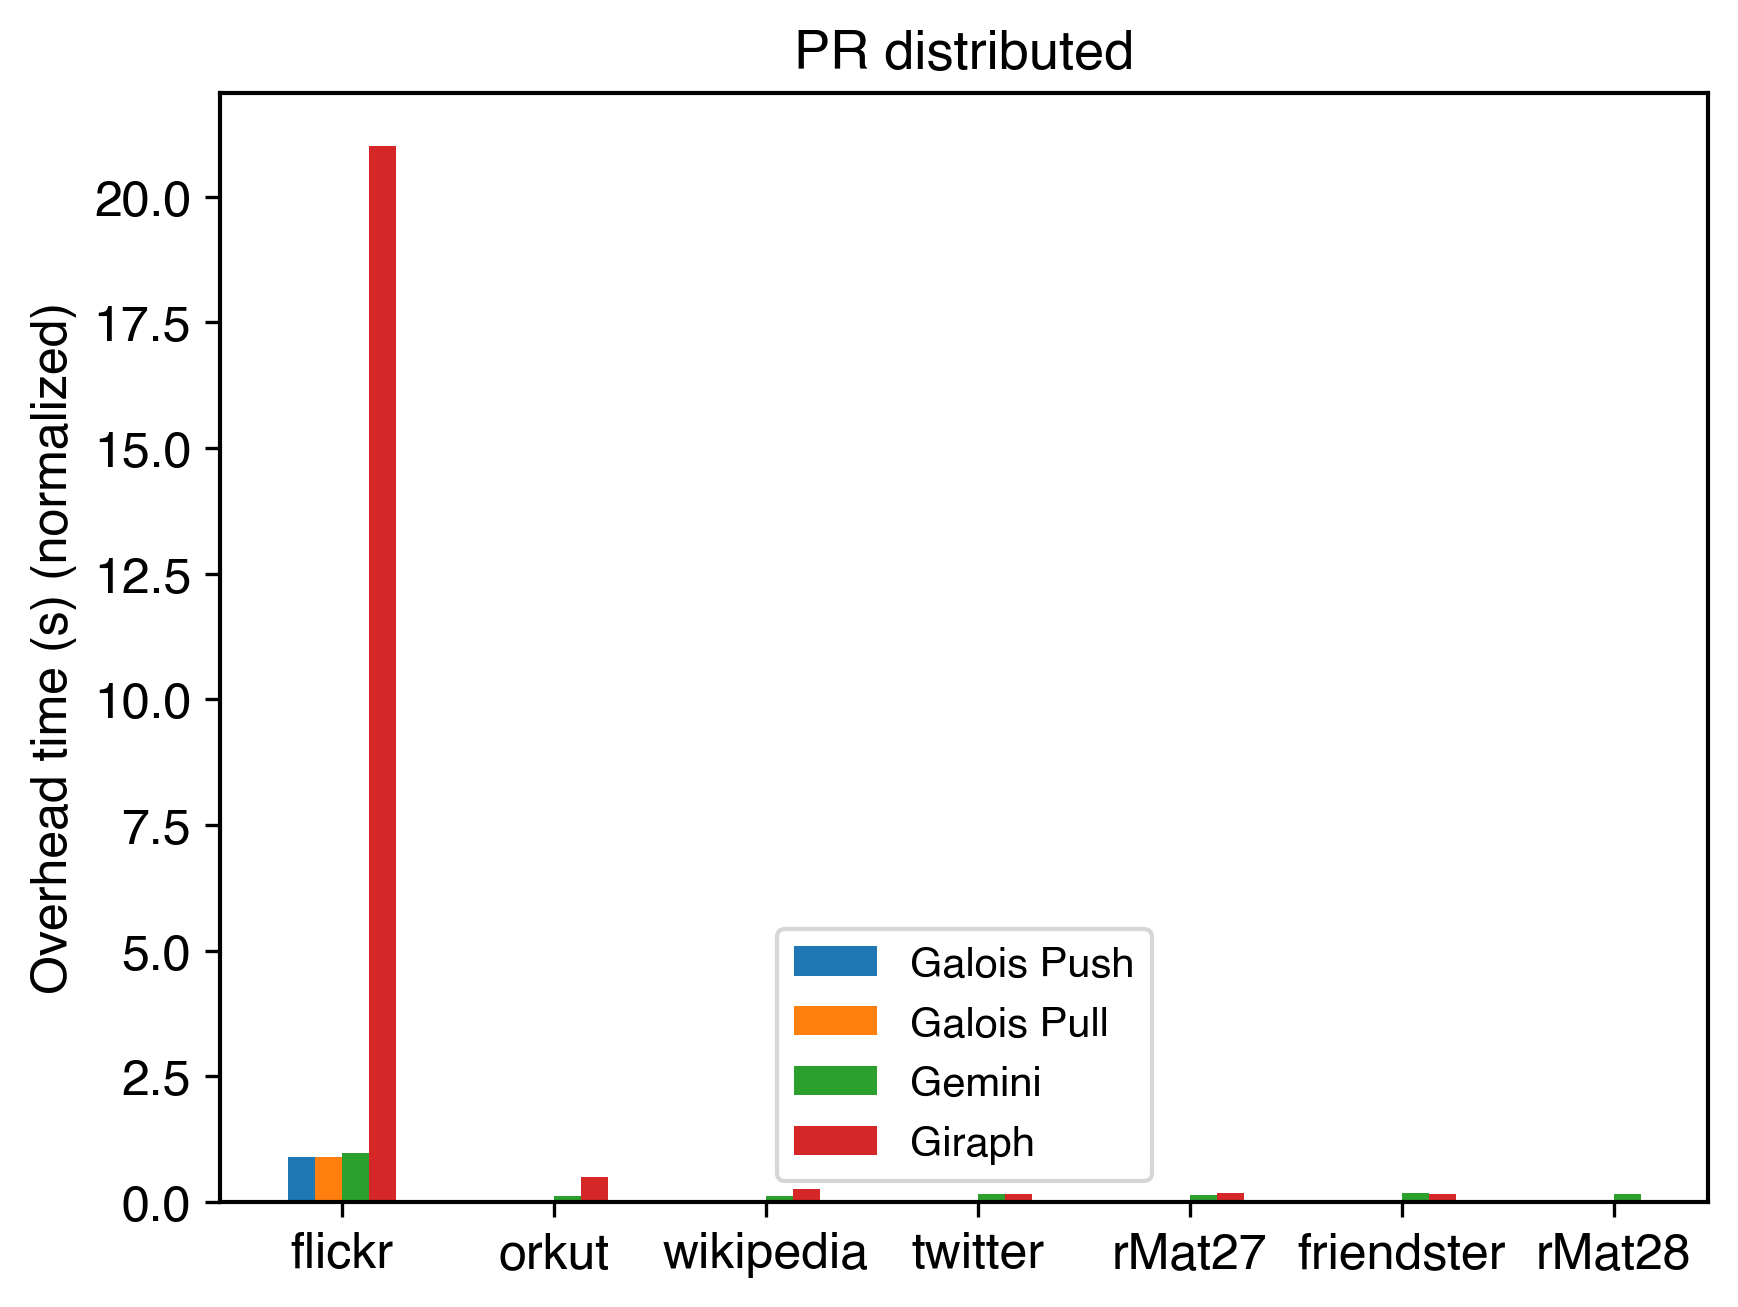
\includegraphics[width=\linewidth]{../../plots/distributedPR_overheadTimeNormalized.png}
		\caption{Overhead time normalized by the graph size in million edges}
		\label{fig:distributedPR_overheadNormalized}
	\end{subfigure}
	
	\caption{Average times on the distributed cluster, black bars represent one standard deviation in our testing}
\end{figure*}









